\subsection{Tensorstruktur}

% Definition Masse und Laplace Matrix
\begin{frame}

\begin{framed}
\textbf{Lokale Massenmatrix}
\begin{equation*} \label{eq:mass}
M_{ik} = \int\limits_{T} \varphi_i (\bold{x}) \, \varphi_j (\bold{x}) \, d\bold{x}
\end{equation*}

\textbf{Elementsteifigkeitsmatrix der Laplace Bilinearform}
\begin{equation*}
V_{ij} = \int\limits_{T} \nabla \varphi_i(\bold{x}) \, \nabla \varphi_j(\bold{x})  d \bold{x}
\end{equation*}
\end{framed}

\begin{itemize}
\item $T$ sei die Referenzzelle für Rechtecke
\item $\varphi_i(\bold{x})$ sei eine zweidimensionale reelle Basisfunktion des diskreten Raumes $V_n$ mit $\bold{x}=(x,y)$ .
\end{itemize}

\end{frame}



% Tensorstruktur der Ansatzfunktionen
\begin{frame}
\frametitle{Tensorstruktur der Ansatzfunktionen}

\begin{equation*} \label{eq:tensor}
\varphi^{2D}_i(\bold{x})=\varphi^{2D}_{i_1+(N+1)i_2}(x,y)=\varphi^{1D}_{i_1}(x)\varphi^{1D}_{i_2}(y),
\end{equation*}

\begin{figure}[ht] 
	\centering
  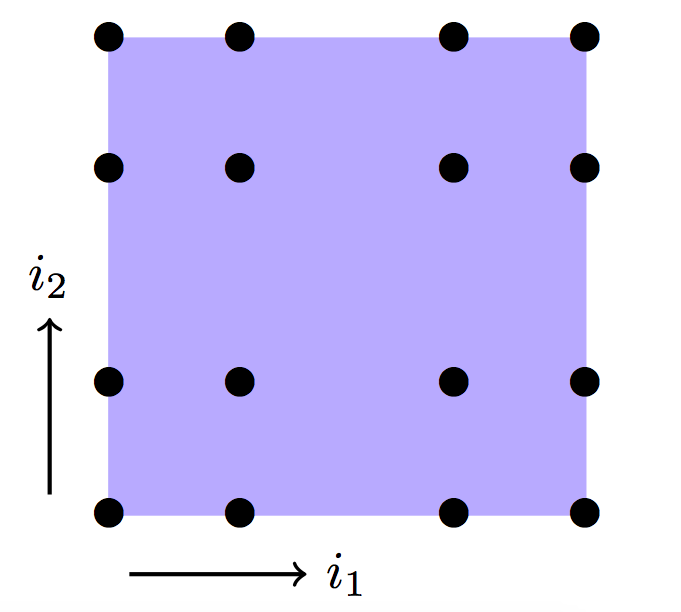
\includegraphics[width=0.3\textwidth]{lexi.png}
	\caption{ \cite[3]{Teachlet}}
	\label{fig:lexi}
\end{figure}

\center{\textbf{Ziel} Definiere Index-Transformation $p$, sodass $p(i)=(i_1,i_2)$.}

\end{frame}

\begin{frame}
\frametitle{Index-Transformation}
Das Inverse der Transformation ist gegeben durch
\begin{equation} \label{eq:tupel}
p^{-1}(i_1,i_2) = i_1 + (N+1)i_2 = i \, 
\end{equation}

\textbf{Extrahiere $i_1$} durch

\begin{equation*}
\begin{aligned}
i \, \, (mod (N+1)) &=p^{-1}(i_1,i_2) \, \, (mod (N+1)) \\ &= i_1 + \underbrace{(N+1)i_2}_{0} \, \, \, (mod (N+1)) \\ &= i_1
\end{aligned}
\end{equation*}

\textbf{Nutze} (\ref{eq:tupel}) um $i_2$ zu erhalten
\begin{equation*} \label{eq:tupel2}
 i_2 = \dfrac{ i - i_1 } {N+1}.
\end{equation*}
\end{frame}

\begin{frame}
\frametitle{Index-Transformation}
\begin{framed}
\begin{equation*} \label{eq:p}
p(i)= \Big{(} i \, \, (mod (N+1)),  \dfrac{ i -  (i \, \, (mod (N+1))) } {N+1} \Big{)}
\end{equation*}
\end{framed}
\end{frame}

\begin{frame}
\frametitle{Tensorstruktur der Massenmatrix}
Es seien $\bold{x}_q=(x_{q1},x_{q2})$ die Stützstellen und $\bold{w}_q=w_{q1}w_{q2}$ die Gewichte der Gauss Quadratur.
\begin{equation*} \label{eq:massapprox}
\begin{aligned}
M_{ij} &= \int\limits_{T} \varphi_i (\bold{x}) \, \varphi_j (\bold{x}) \, d\bold{x} \\ \pause
&\approx  \sum\limits_{q=1}^Q \bold{w}_q \, \, \varphi_i (\bold{x}_q) \, \varphi_j (\bold{x}_q) \\ \pause
&= \sum\limits_{q_1=1}^{Q_{1D}} \sum\limits_{q_2=1}^{Q_{1D}} \varphi_{i_1}(x_{q1}) \varphi_{i_2}(x_{q2}) \varphi_{j_1}(x_{q1}) \varphi_{j_2}(x_{q2}) \, w_{q1} w_{q2} \\ 
&= \sum\limits_{q_1=1}^{Q_{1D}} w_{q1} \varphi_{i_1}(x_{q1}) \varphi_{j_1}(x_{q1}) \sum\limits_{q_2=1}^{Q_{1D}} w_{q2} \varphi_{i_2}(x_{q2}) \varphi_{j_2}(x_{q2}) \, . 
\end{aligned}
\end{equation*}
\end{frame}

\begin{frame}
\textbf{Definiere} \\
\begin{itemize}
\item Es sei $\mathcal{N}$ eine Matrix mit $\mathcal{N}_{iq}=\varphi_i(\bold{x}_q)$.
\item Es sei $\mathcal{W}$ eine Matrix mit $\mathcal{W}_{ii}=\bold{w}_i$, sonst Nullen.
\end{itemize}
Dann können wir die Massenmatrix schreiben als
\begin{equation*}
M = \underbrace{\mathcal{N} \mathcal{W}}_{:=\mathcal{W}_N} \mathcal{N}^T. = \mathcal{W}_N \mathcal{N}^T
\end{equation*}
\pause
\textbf{Nutze Tensorstruktur der Ansatzfunktionen}
\begin{equation*}
\begin{aligned}
\mathcal{N} &= \mathcal{N}^{1D} \otimes \mathcal{N}^{1D} \\
\mathcal{W}_N &= \mathcal{W}_N^{1D} \otimes \mathcal{W}_N^{1D}
\end{aligned}
\end{equation*}
\end{frame}

\begin{frame}
\frametitle{Tensorstruktur der Massenmatrix}
\begin{framed}
\begin{equation*}
\begin{aligned}
M &= \mathcal{W}_N \mathcal{N}^T \\
&= (\mathcal{W}_N^{1D} \otimes \mathcal{W}_N^{1D})(\mathcal{N}^{1D} \otimes \mathcal{N}^{1D})^T \\
&= (\mathcal{W}_N^{1D} \otimes \mathcal{W}_N^{1D})((\mathcal{N}^{1D})^T \otimes (\mathcal{N}^{1D})^T) \\
&= (\mathcal{W}_N^{1D} (\mathcal{N}^{1D})^T) \otimes  (\mathcal{W}_N^{1D} (\mathcal{N}^{1D})^T) 
\end{aligned}
\end{equation*}
\end{framed}
\end{frame}

\begin{frame}
\frametitle{Pseudoinverse der Massenmatrix}
\begin{equation*}
\begin{aligned}
M^+ & = [(\mathcal{W}_N^{1D} (\mathcal{N}^{1D})^T) \otimes  (\mathcal{W}_N^{1D} (\mathcal{N}^{1D})^T)]^+ \\ &= (\mathcal{W}_N^{1D} (\mathcal{N}^{1D})^T)^+ \otimes  (\mathcal{W}_N^{1D} (\mathcal{N}^{1D})^T)^+ 
\end{aligned}
\end{equation*}
\end{frame}





\begin{frame}
\frametitle{Tensorstruktur der Laplace Bilinearform}
\begin{equation*}
\begin{aligned}
V_{ij} &= \int\limits_{T} \nabla \varphi_i(\bold{x}) \, \nabla \varphi_j(\bold{x})  d \bold{x} \\ 
&= \int\limits_{T}( \partial_{x_1}  \varphi_i(\bold{x})  \partial_{x_1} \varphi_j(\bold{x})) + ( \partial_{x_2} \varphi_i(\bold{x})  \partial_{x_2} \varphi_j(\bold{x})) \, d\bold{x} \\
&= \int\limits_{T}( \partial_{x_1}  \varphi_i(\bold{x})  \partial_{x_1} \varphi_j(\bold{x})) + ( \partial_{x_2} \varphi_i(\bold{x})  \partial_{x_2} \varphi_j(\bold{x})) \, d\bold{x} \\ &= \int\limits_{T} \partial_{x_1}  \varphi_i(\bold{x})  \partial_{x_1} \varphi_j(\bold{x}) d\bold{x} + \int\limits_{T}  \partial_{x_2} \varphi_i(\bold{x})  \partial_{x_2} \varphi_j(\bold{x}) \, d\bold{x} \\
&= \underbrace{\sum\limits_{q=1}^{(N+1)^2} \bold{w}_q \partial_{x_1}  \varphi_i(\bold{x}_q)  \partial_{x_1} \varphi_j (\bold{x}_q)}_{K^1} + \underbrace{\sum\limits_{q=1}^{(N+1)^2} \bold{w}_q  \partial_{x_2} \varphi_i(\bold{x}_q)  \partial_{x_2} \varphi_j(\bold{x}_q)}_{K^2} \, 
\end{aligned}
\end{equation*}
\end{frame}

\begin{frame}
\begin{equation*}
\begin{aligned}
K_{ij}^1 &=\sum\limits_{q=1}^{(N+1)^2} \bold{w}_q \partial_{x_1}  \varphi_i(\bold{x}_q)  \partial_{x_1} \varphi_j (\bold{x}_q) \\ &= \sum\limits_{q_1=1}^{N} \sum\limits_{q_2=1}^{N} w_{q1}w_{q2} \partial_{x_1}  \varphi_{i1}(x_{q1})\varphi_{i2}(x_{q2})  \partial_{x_1} \varphi_{j1} (x_{q1})\varphi_{j2} (x_{q2}) \\
&=  \sum\limits_{q_1=1}^{N} \sum\limits_{q_2=1}^{N} w_{q1}w_{q2} \varphi'_{i1}(x_{q1})\varphi_{i2}(x_{q2})  \varphi'_{j1} (x_{q1})\varphi_{j2} (x_{q2}) \\ 
&= \sum\limits_{q_1=1}^{N} w_{q1} \varphi'_{i1}(x_{q1}) \varphi'_{j1} (x_{q1}) \sum\limits_{q_2=1}^{N} w_{q2} \varphi_{i2}(x_{q2})  \varphi_{j2} (x_{q2}) 
\end{aligned}
\end{equation*}
\end{frame}

\begin{frame}
\textbf{Definiere}
\begin{itemize}
\item Es sei $\widehat{\mathcal{N}}^{1D}$ eine Matrix mit $\widehat{\mathcal{N}}^{1D}_{ik}=\varphi'^{1D}_i(x_k)$
\item Dementsprechend ist $\widehat{\mathcal{W}}^{1D}_N$ eine Matrix, die aufgebaut ist wie $\mathcal{W}^{1D}_N$, mit dem Unterschied, dass sie die Evaluationen der ersten Ableitungen der Ansatzfunktionen beinhaltet.
\end{itemize}
\pause
\textbf{Dann} können wir $K_1,K_2$ schreiben als
\begin{align*}
K_1 &= (\widehat{\mathcal{W}}_N^{1D} (\widehat{\mathcal{N}}^{1D})^T) \otimes (\mathcal{W}_N^{1D}(\mathcal{N}^{1D})^T) \\
K_2 &= (\mathcal{W}_N^{1D} (\mathcal{N}^{1D})^T) \otimes (\widehat{\mathcal{W}}_N^{1D} (\widehat{\mathcal{N}}^{1D})^T)
\end{align*}
\begin{framed}
\begin{equation*}
V =\widehat{\mathcal{W}}_N \widehat{\mathcal{N}}^T \otimes \mathcal{W}_N \mathcal{N}^{T} + \mathcal{W}_N \mathcal{N}^{T}\otimes \widehat{\mathcal{W}}_N \widehat{\mathcal{N}}^T.
\end{equation*}
\end{framed}
\end{frame}

\begin{frame}
\frametitle{Problem bei Laplace}
\textbf{Problem } Die Addition in der Tensorstruktur macht unseren ersten Ansatz hinfällig. \\
\textbf{Idee } Vereinfache die Form durch geeignete Basiswahl und dann sehen wir weiter. Wir wählen geeignete Basis, sodass $ \, \mathcal{W}_N \mathcal{N}^{T} = I_n \, $.

Folgende Basispolynome bieten sich an:
\begin{framed}
\begin{equation*}
\varphi^{1D}_i (x_k) = \dfrac{1}{ \sqrt{w_i} } l_i (x_k) = 
\begin{cases}
\dfrac{1}{ \sqrt{w_i} } \, \text{ , wenn } i=k  \\
0  \, \, \, \, \, \, \, \, \, \, \, \text{ , sonst. }
\end{cases}
\end{equation*}
Die Funktion $l_i(x_k)$ bezeichnet das $i-te$ Lagrange Polynom.
\end{framed}
\end{frame}

\begin{frame}
\begin{framed}
\textbf{Zeige} 
\begin{equation*}
\mathcal{W}_N^{1D} (\mathcal{N}^{1D})^T = \mathcal{N}^{1D} \mathcal{W}^{1D} (\mathcal{N}^{1D})^T = I_n
\end{equation*}
\end{framed}
\begin{itemize}
\item $\mathcal{N}$ ist Diagonalmatrix mit Einträgen $\dfrac{1}{ \sqrt{w_i} }$
\item Es gilt $\mathcal{N}=\mathcal{N}^T$. 
\item $\mathcal{W}$ Diagonalmatrix mit Einträgen $w_i$ in der Diagonalen.
\end{itemize}
In der Ergebnismatrix steht dann in der Diagonalen 
\begin{equation*}
(\dfrac{1}{ \sqrt{w_i} })^2  w_i = 1 \, ,
\end{equation*}
sonst Nullen.
\end{frame}

\begin{frame}
\begin{itemize}
\item Definiere $A:=\widehat{\mathcal{W}}_N^{1D} (\widehat{\mathcal{N}}^{1D})^T$.
\item Wähle Basis so, dass $\mathcal{W}_N^{1D} (\mathcal{N}^{1D})^T  = I_n$ gilt.
\end{itemize}
Dann können wir das Matrix-Vektor Produkt $Vu$ darstellen durch
\begin{equation*} \label{eq:easy}
y=Vu =[(A \otimes I_n) + (I_n \otimes A)]u.
\end{equation*}
\pause
\textbf{Transformiere} u und y zu Matrizen $U$ und $Y$ mit Hilfe der Index-Transformation $p(\cdot)$.
\begin{equation*} \label{eq:easy}
Y=VU =[(A \otimes I_n) + (I_n \otimes A)]U=AUI_n^T + I_nUA^T=AU+UA^T.
\end{equation*}
\pause
\begin{framed}
\center{\textbf{Lyapunow Gleichung}} \\
\begin{equation*}
Y=AU+UA^T.
\end{equation*}
\end{framed}
\end{frame}

\subsection{Pseudoinverse durch Singulärwertzerlegung höherer Ordnung}
\begin{frame}

\textbf{Lokaler Massetensor}
\begin{equation*} 
M_{i1,i2,j1,j2} = \int\limits_{T} \varphi_{i1} (x_1) \varphi_{i2}(x_2) \varphi_{j1} (x_1) \varphi_{j2} (x_2) \, d(x_1,x_2)
\end{equation*}

\textbf{Lokaler Laplace Tensor}
\begin{equation*} 
\begin{aligned}
V_{i1,i2,j1,j2} = \int\limits_{T} \varphi'_{i1} (x_1) \varphi_{i2}(x_2) &\varphi'_{j1} (x_1) \varphi_{j2} (x_2) + \\
&\varphi_{i1} (x_1) \varphi'_{i2}(x_2) \varphi_{j1} (x_1) \varphi'_{j2} (x_2) \, d(x_1,x_2).
\end{aligned}
\end{equation*} \\
$\rightarrow$ Was ist die Pseudoinverse eines Tensors?
\end{frame}

\begin{frame}
\frametitle{Moore Penrose Pseudoinverse}
\begin{framed}
\textbf{Definition} (Moore Penrose Pseudoinverse) 
\begin{enumerate}
\item $AA^{+}A \, \, \, \, \,  =A$
\item $A^{+}AA^{+} \, \, =A^{+}$ 
\item $(AA^{+})^{T} \, \,  =AA^{+}$
\item $(A^{+}A)^{T} \, \, =A^{+}A$ 
\end{enumerate}
\end{framed}
\textbf{Probleme}
\begin{enumerate}
\item Wir haben kein Tensor-Tensor Produkt.
\item Wir wissen nicht was die Transponierte eines Tensors ist.
\end{enumerate}
\end{frame}

\begin{frame}
\frametitle{Tensor Operationen}
\begin{framed} \textbf{Definition} (Tensor-Tensor Produkt) \\
Es seien $\pmb{\mathcal{X}}^1  \in \mathbb{R}^{I_1 \times I_2 \times I_1 \times I_2}$ und $\pmb{\mathcal{X}}^2 \in \mathbb{R}^{I_1 \times I_2 \times I_1 \times I_2}$ Tensoren.
Dann definieren wir das Produkt dieser beiden Tensoren elementweise wie folgt
\begin{equation}
ttp(\pmb{\mathcal{X}}^1,\pmb{\mathcal{X}}^2)_{i_1,i_2,j_1,j_2}= \sum_{j_1=1}^{I_1} \sum_{j_2=1}^{I_2} \pmb{\mathcal{X}}^1_{i_1,i_2,j_1,j_2} \pmb{\mathcal{X}}^2_{j_1,j_2,k_1,k_2} 
\end{equation}
\end{framed}
\end{frame}

\begin{frame}
\frametitle{Tensor Operationen}
\begin{framed} \textbf{Definition} (Transponierte eines Tensors) \\
Es seien $\pmb{\mathcal{X}} \in \mathbb{R}^{I_1 \times I_2 \times I_1 \times I_2}$ ein Tensor.
Dann definieren wir die Transponierte des Tensors elementweise wie folgt
\begin{equation*}
\mathcal{X}_{i_1 \, i_2 \, i_1 \, j_2}^T = \mathcal{X}_{p^{-1}(i_1,i_2)p^{-1}(j_1,j_2)}^T=\mathcal{X}_{p^{-1}(j_1,j_2)p^{-1}(i_1,i_2)} =\mathcal{X}_{ j_1 \, j_2 \, i_1 \, i_2}
\end{equation*}
\end{framed}
\end{frame}


\begin{frame}
\frametitle{Moore Penrose Pseudoinverse für Tensoren}
\begin{framed} \textbf{Definition} (Moore Penrose Pseudoinverse für Tensoren) \\
\begin{enumerate}
\item $ttp(A,ttp(A^{+},A))-A \, \, \, \, \, \, \, \, \, \, \, = 0$
\item $ttp(A^{+},ttp(A,A^{+}))-A^{+} \, \,  \, \, = 0 $
\item $(ttp(A,A^{+}))^{T}-ttp(A,A^{+}) = 0$
\item $(ttp(A^{+},A))^{T}-ttp(A^{+},A) = 0$
\end{enumerate}
\end{framed}
\end{frame}

\begin{frame}
\frametitle{Pseudoinverse der HOSVD}
\center{
Die HOSVD eines Tensors $\pmb{\mathcal{X}}  \in \mathbb{R}^{I_1 \times I_2 \times I_3 \times I_4}$  ergibt
\begin{equation*}
\pmb{\mathcal{X}} = \pmb{\mathcal{G}} \times_{n=1}^{4} U^{ (n) }.
\end{equation*}
Die Pseudoinverse des Tensors $\mathcal{X}$ erhält man über}
\begin{framed}
\begin{equation*} 
\pmb{\mathcal{X}}^{+} = \pmb{\mathcal{G}}^{+} \times_{n=1}^{4} U^{ (n) ^{T} }.
\end{equation*}
\end{framed}

\end{frame}